% m1_outcomes_parameters.tex
% Purpose: Expanded M1 "Expected Outcomes" (Sec. VI) and "Simulation Parameters"
%          (Appendix A) in IEEEtran format. Values are the actual calibrated
%          defaults from src/main/resources/simulation.properties and the
%          measured M4 baseline results (documents/m4/*.csv).
% TODO before submission:
%   - Paste \section{Expected Outcomes} and the \appendix block into the main M1 .tex,
%     replacing the existing Section VI, Appendix A, and Appendix B.
%   - Appendix B text is revised to match the implemented diagrams
%     (documents/Classdiagram.puml, documents/ActivityUML.puml).
%   - Confirm reference keys (\cite) match the main document's bibliography.
%   - This file also compiles standalone for a quick preview.

\documentclass[conference]{IEEEtran}
\usepackage{amsmath}
\usepackage{booktabs}
\usepackage{array}
\usepackage{graphicx}
% Look for figures in ./figures and the project root, so uploads work either way.
\graphicspath{{figures/}{./}}
\begin{document}

% ---------------------------------------------------------------------------
% Section VI: Expected Outcomes
% ---------------------------------------------------------------------------
\section{Expected Outcomes}
This project targets a small set of outcomes drawn from direct dealership
experience, each stated as a testable prediction against the simulation's
tracked metrics. The M4 analysis batch (30 replications, seeds 42--71) is
referenced where it already confirms or qualifies a prediction.

\subsection{Staffing and throughput follow a diminishing-returns curve}
Adding technicians and bays should raise throughput and cut customer wait,
but only until advisor intake becomes the binding constraint. Beyond that
point, extra technicians add cost without adding utilization. The baseline
configuration ($\lambda = 4$, $c = 3$, four advisors) is expected to sit in a
moderate-load regime rather than at saturation; the analytical M/M/c check
gives $\rho = 0.667$ and $W_q = 0.222$~h for reference. Moving from three to
five technicians is expected to shorten wait modestly while pushing
utilization down, the signature of spare capacity rather than added output.

\subsection{Parts delay decouples wait from utilization}
A longer or more variable parts lead time should inflate total wait while
leaving technician utilization near its baseline level. This is the
``phantom under-utilization'' case: a vehicle occupies a bay, but no
value-adding work is in progress because the job is blocked on parts. The
metric to watch is $D_{\text{parts}}$ rising sharply while jobs completed and
utilization stay close to baseline, which separates a supply-chain problem
from a staffing problem.

\subsection{The morning rush sets the day's worst queue}
Because arrivals follow a time-of-day rush curve (the \texttt{DEALERSHIP\_DAY}
profile) rather than a flat rate, the first arrival surge is expected to
create the longest single backlog of the day. Since the earliest shift is
typically the leanest, wait time should peak early and then relax as capacity
catches up. Under the peak scenario ($\lambda = 8$) the model is expected to
absorb the extra volume at the cost of higher wait and utilization rather
than by dropping jobs.

\subsection{Wait time is the most parameter-sensitive metric}
Of the tracked outputs, mean total customer wait $W_{\text{total}}$ is
expected to respond most strongly to changes in service rate $\mu$ and
technician count $c$, more so than to arrival rate over the tested range.
Utilization is expected to track load closely, while jobs completed should
stay near the arrival-driven ceiling except under saturation. These
directional responses are the primary target of the M4 sensitivity and
scenario testing.

% ---------------------------------------------------------------------------
% Appendix A: Simulation Parameters
% ---------------------------------------------------------------------------
\appendices
\section{Simulation Parameters}
Table~\ref{tab:params} lists the calibrated default configuration used for the
baseline runs. These values are the shipped defaults in
\texttt{simulation.properties}; per-experiment sweeps in M4 vary one parameter
at a time around this baseline. Values previously marked ``TBD'' in the M1
proposal are now fixed to the implemented defaults.

\begin{table}[h]
\centering
\caption{Baseline Simulation Input Parameters}
\label{tab:params}
\renewcommand{\arraystretch}{1.2}
\begin{tabular}{@{}p{3.1cm}cp{2.6cm}@{}}
\toprule
\textbf{Parameter} & \textbf{Symbol} & \textbf{Value} \\
\midrule
Customer arrival rate & $\lambda$ & 4.0 veh/h \\
Arrival profile & --- & \texttt{DEALERSHIP\_DAY} (Cox) \\
Mean service time / tech & $1/\mu$ & 0.5 h ($\mu = 2.0$/h) \\
Technicians / bays & $c$ & 3 \\
Service advisors & --- & 4 \\
Experience level (norm.) & $e_i$ & $[0,1]$, raw $0$--$E_{\max}$ \\
Max experience level & $E_{\max}$ & 10 \\
Experience coefficient & $\alpha$ & 1.0 \\
Gamma shape parameter & $k$ & 4.0 \\
Parts reorder point & $r$ & 5 units \\
Parts reorder quantity & $Q$ & 10 units \\
Initial parts on hand & --- & 20 units \\
Parts lead time & $L$ & 2.0 h (stochastic) \\
Simulation run length & --- & 10 h (1 work day) \\
Replications & --- & 30 (seeds 42--71) \\
Random seed (base) & --- & 42 \\
Validation tolerance & --- & 0.15 (relative) \\
\bottomrule
\end{tabular}
\end{table}

The experience-based service time uses the normalized level
$e_i = \min(1, e_i^{\text{raw}} / E_{\max})$ in the scaling function
$f(e_i) = 1 / (1 + \alpha e_i)$, so raw levels of $0$--$10$ map onto $[0,1]$
before scaling the mean service time. Service durations are drawn from a Gamma
distribution with shape $k = 4.0$, fixing the mean at $\mu_i$ while controlling
variance independently. The single production default of one replication is
overridden to 30 for the reported statistical batches.

% ---------------------------------------------------------------------------
% Appendix B: UML Diagrams
% ---------------------------------------------------------------------------
\section{UML Diagrams}
Two UML diagrams document the project, both authored in PlantUML and stored in
the repository: the class diagram (\texttt{documents/Classdiagram.puml}) and
the activity diagram (\texttt{documents/ActivityUML.puml}). The descriptions
below reflect the implemented source rather than the original proposal sketch;
notably the ticket entity is named \texttt{ServiceTicket}, and the parts logic
is owned by a \texttt{PartsDepartment} class. Both diagrams are rendered from
the PlantUML source and embedded in Fig.~\ref{fig:class} and
Fig.~\ref{fig:activity}.

\begin{figure*}[t]
\centering
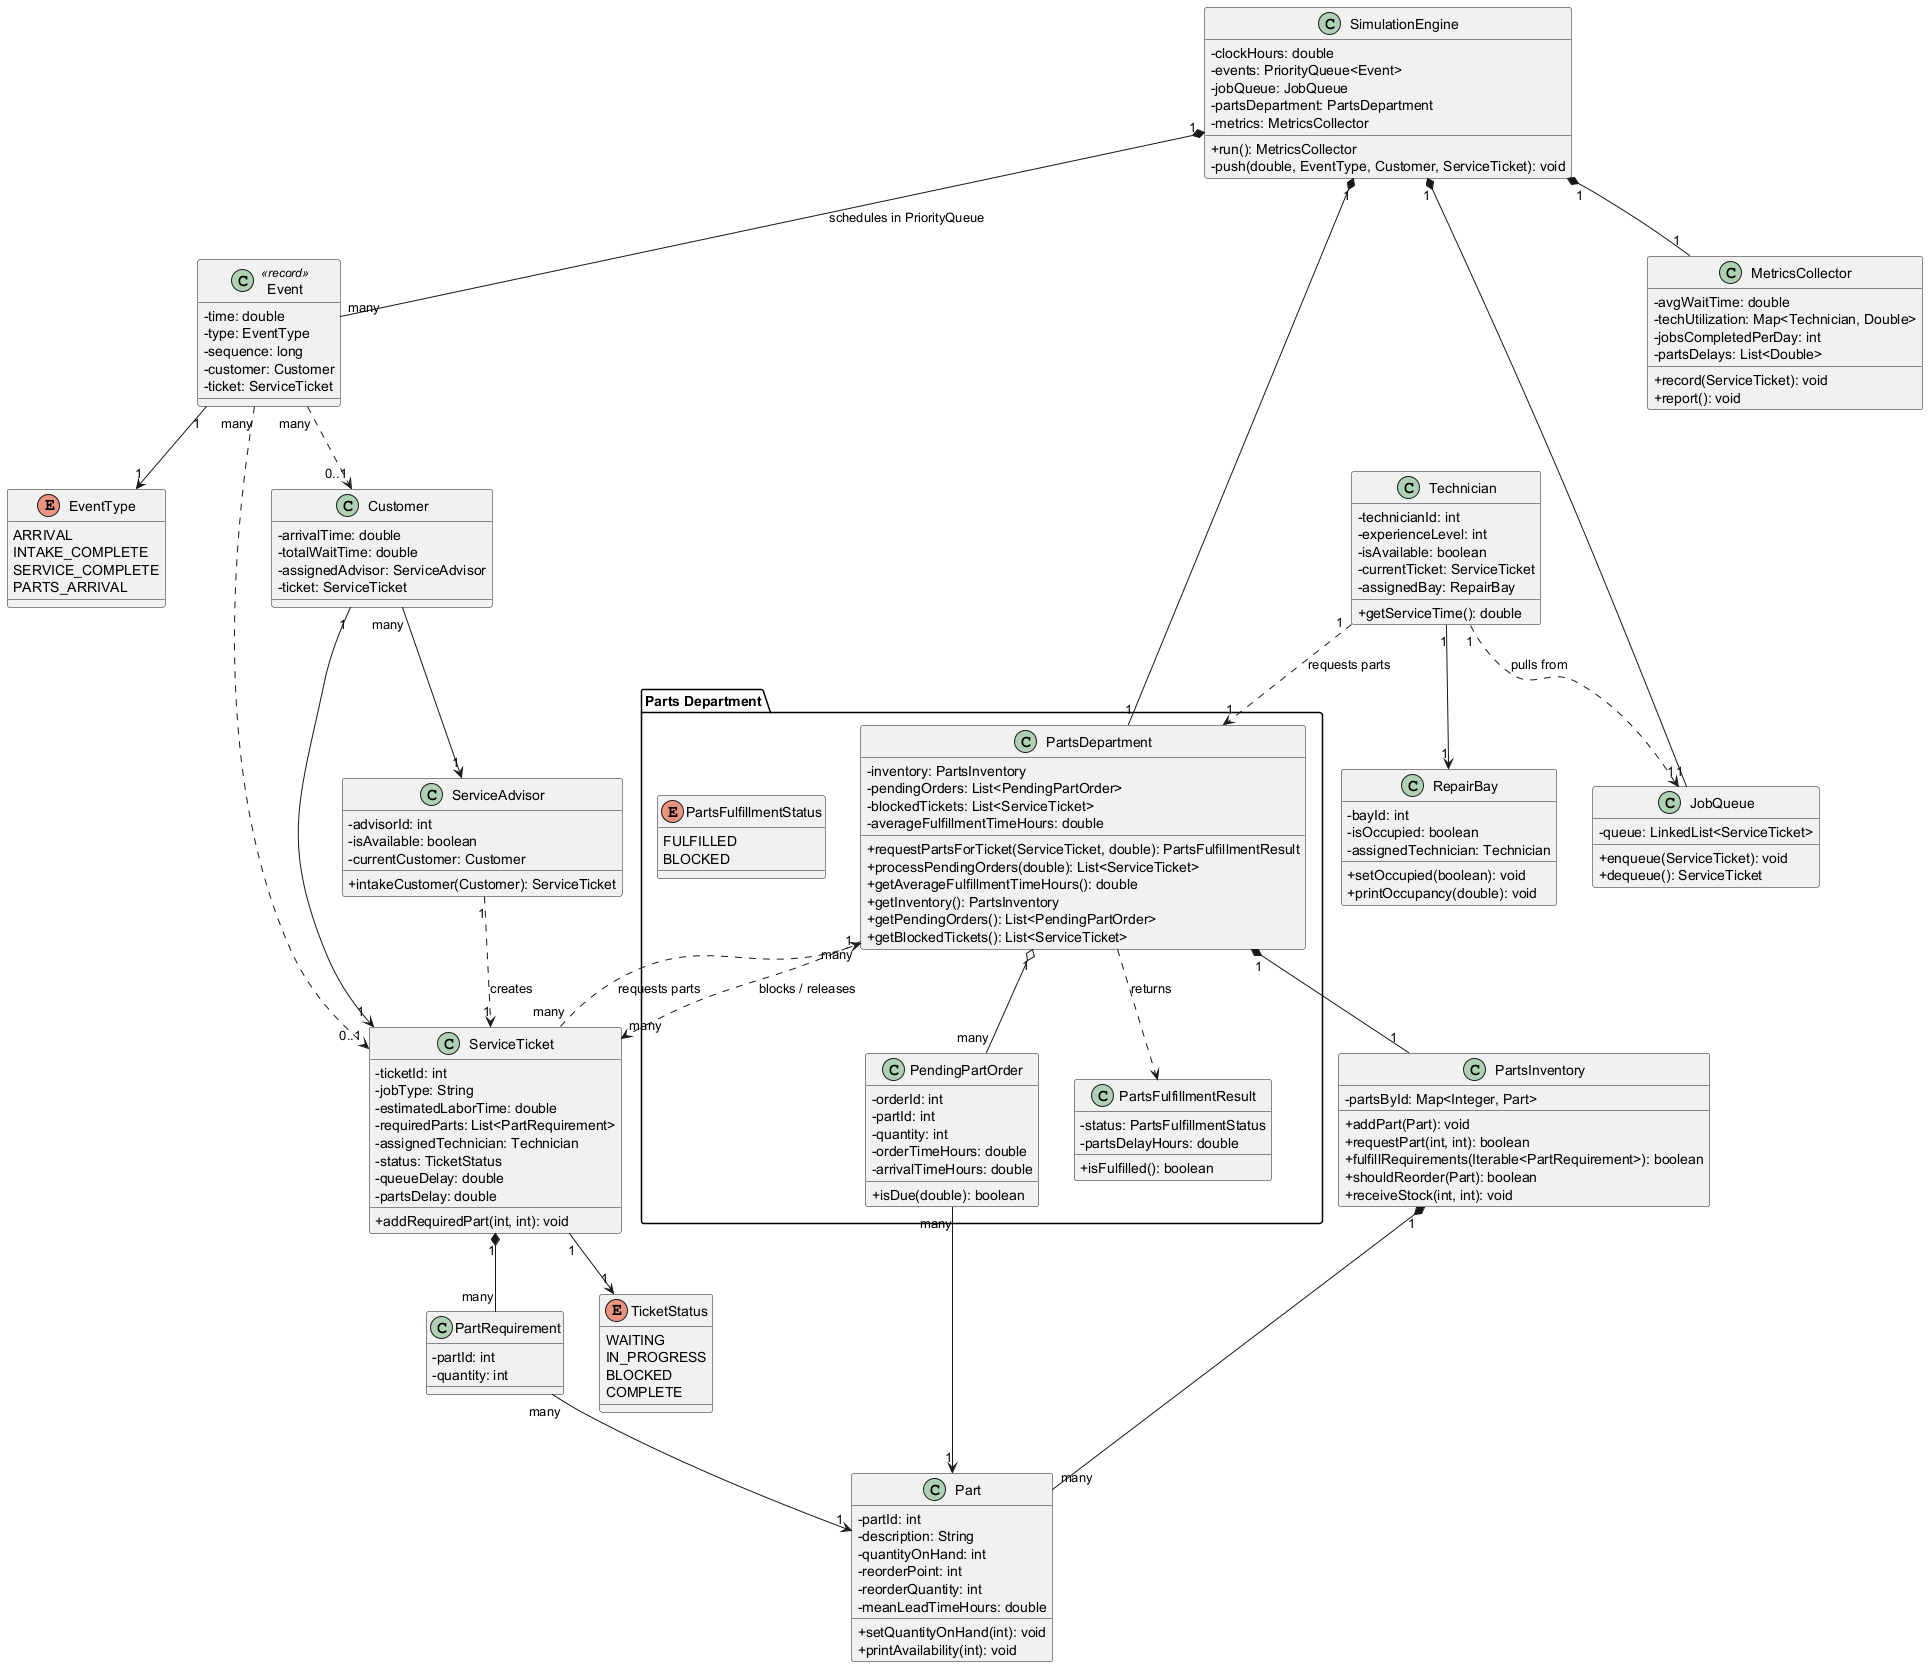
\includegraphics[width=\textwidth]{figures/ClassDiagram.png}
\caption{Class diagram rendered from \texttt{documents/Classdiagram.puml}.}
\label{fig:class}
\end{figure*}

\begin{figure*}[t]
\centering
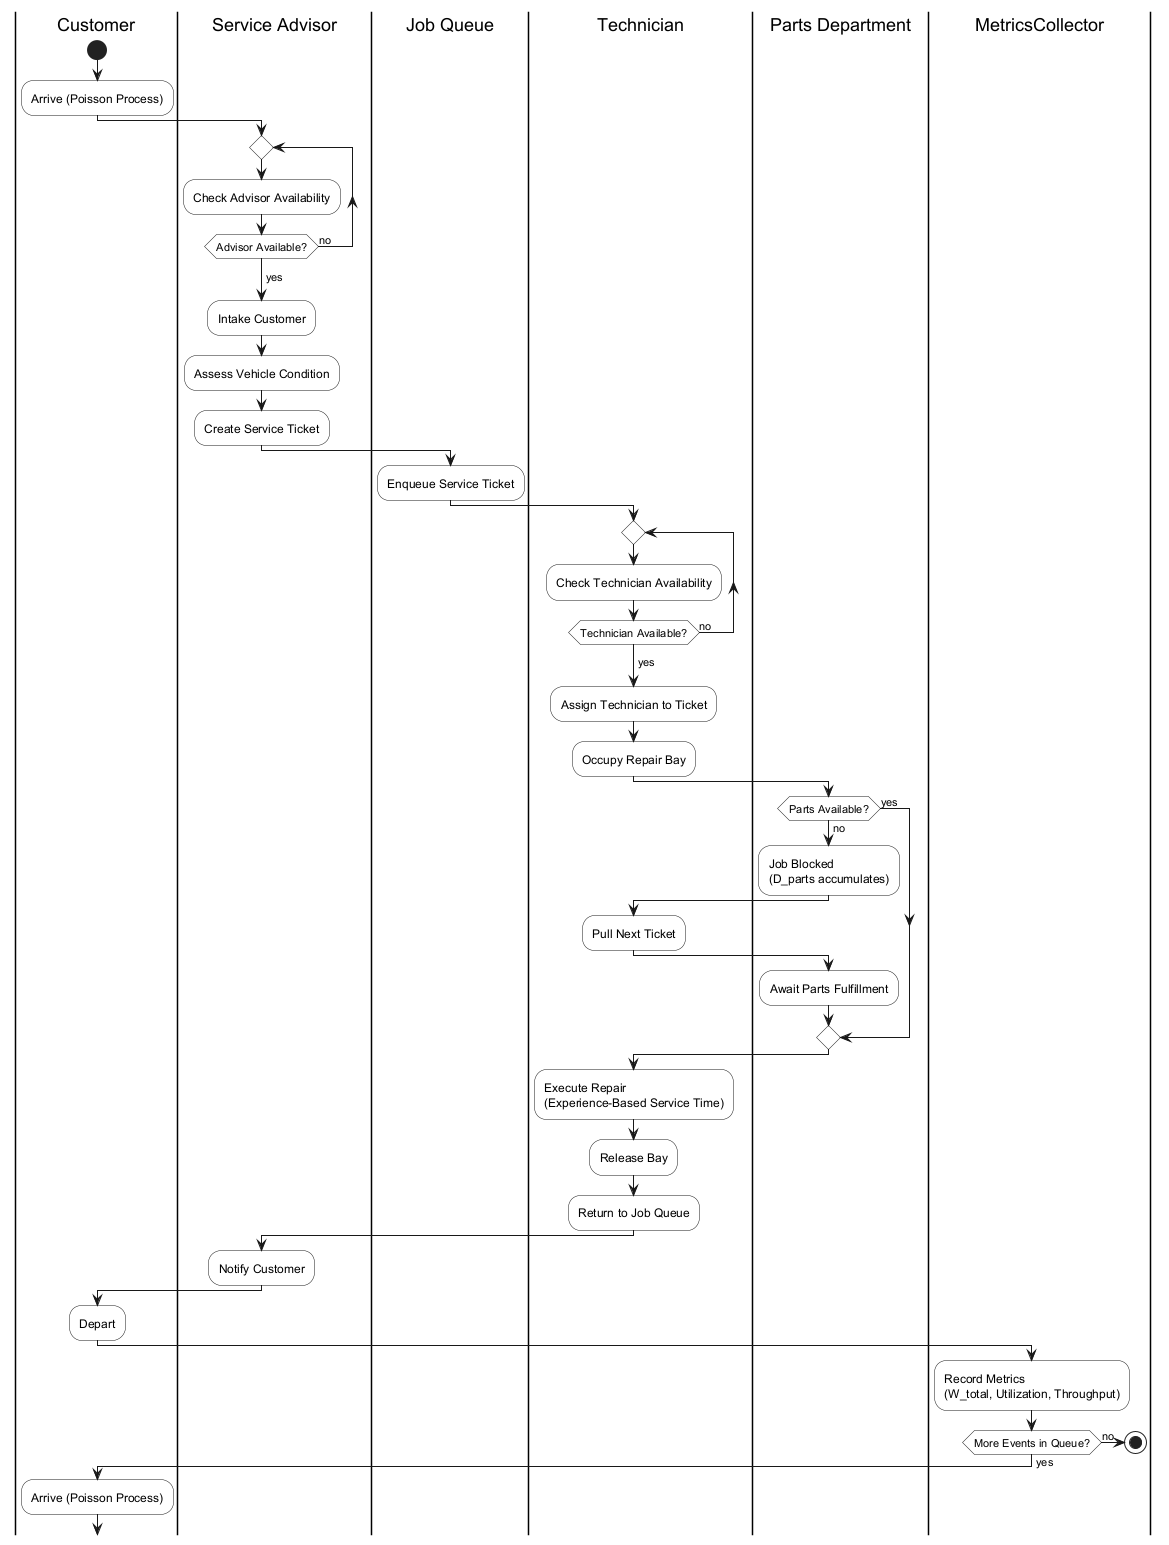
\includegraphics[height=0.9\textheight]{figures/ActivityDiagram.png}
\caption{Activity diagram rendered from \texttt{documents/ActivityUML.puml}.}
\label{fig:activity}
\end{figure*}

\subsection{Class Diagram}
The class diagram is organized around a discrete-event core. The
\texttt{SimulationEngine} owns the event loop, scheduling \texttt{Event}
records in a priority queue ordered by (time, sequence) and dispatching them by
\texttt{EventType} (\texttt{ARRIVAL}, \texttt{INTAKE\_COMPLETE},
\texttt{SERVICE\_COMPLETE}, \texttt{PARTS\_ARRIVAL}). The engine composes the
\texttt{JobQueue}, \texttt{MetricsCollector}, and \texttt{PartsDepartment}.

The domain entities are \texttt{Customer}, \texttt{ServiceAdvisor},
\texttt{ServiceTicket} (with its \texttt{PartRequirement} list and
\texttt{TicketStatus} of \texttt{WAITING}, \texttt{IN\_PROGRESS},
\texttt{BLOCKED}, or \texttt{COMPLETE}), \texttt{Technician}, and
\texttt{RepairBay}. A customer holds one ticket and is assigned to an advisor;
the advisor creates the ticket; each technician maps to one bay, pulls from the
shared \texttt{JobQueue}, and requests parts.

Parts handling is grouped in a dedicated package. \texttt{PartsDepartment}
composes a \texttt{PartsInventory} of \texttt{Part} objects, tracks
\texttt{PendingPartOrder} replenishments, blocks and releases tickets, and
returns a \texttt{PartsFulfillmentResult} (status \texttt{FULFILLED} or
\texttt{BLOCKED}). Relationships use composition for engine- and
department-owned collaborators and dependencies for the transient
request/block/release interactions.

\subsection{Activity Diagram}
The activity diagram traces one vehicle from arrival to departure across six
swimlanes: Customer, Service Advisor, Job Queue, Technician, Parts Department,
and MetricsCollector. A customer arrives under the Poisson/Cox process and
waits until an advisor is available; the advisor intakes the customer, assesses
vehicle condition, and creates a service ticket, which is enqueued in the job
queue. A technician waits for availability, is assigned the ticket, and occupies
a repair bay. Parts availability is a branch: if parts are unavailable the job
is blocked and accrues $D_{\text{parts}}$ while the technician pulls the next
ticket and the parts department awaits fulfillment. Once work proceeds, the
technician executes the repair over an experience-based service time, releases
the bay, and returns to the queue. The advisor notifies the customer, who
departs, and the MetricsCollector records $W_{\text{total}}$, utilization, and
throughput. The flow repeats while events remain, then terminates.

\end{document}
